\documentclass[12pt]{article}
\usepackage[serbian]{babel}
\usepackage {fontspec, amsmath, amssymb, mathtools}
\usepackage {clrscode3e, listings}
\usepackage {graphicx, float, caption, subcaption}

\defaultfontfeatures{Ligatures=TeX}

\addto\captionsserbian{%
  \renewcommand{\abstractname}%
    {Apstrakt}%
}

\let\oldvec\vec
\renewcommand{\vec}[1]{\mathbf{#1}}

\title{Simulacija te\v cnosti u dve dimenzije}
\author{
        Daniel Sila\dj i \\
        Gimnazija "Jovan Jovanovi\'{c} Zmaj"\\
		Novi Sad
}
\date{\today}

\begin{document}
\maketitle

\begin{abstract}
U ovom radu je opisan fizi\v cki i informati\v cki aspekt simulacije fluida (te\v cnosti) pomo\'cu metode \emph{Smoothed Particle Hydrodynamics} (SPH). Iako se opisan algoritam odnosi na dve dimenzije, on se lako mo\v ze generalizovati na tri (pa \v cak i proizvoljan broj) dimenzija. Dobijeni program simulira me\dj usobnu interakciju do oko 10000 \v cestica, kao i njihove sudare sa stati\v cnim zidovima pri brzini od 60 koraka u sekundi (\emph{60fps}) na Intelovom \v cetvorojezgarnom Core i7 procesoru.
\end{abstract}

\section{Uvod}\label{uvod} Simulacije fluida se javljaju na raznim mestima, i to, sa jedne strane u vidu vremenske prognoze, aerodinami\v cki oblikovanih automobila, aviona i raketa, a sa druge strane kao specijalni efekti u filmovima i kompjuterskim igrama.

\label{istorija}
    Prve korake u ovoj oblasti su napravili Claude-Louis Navier i George Gabriel Stokes 1822, postaviv\v si Navier-Stoksove jedna\v cine.
    One \v cine osnovu mnogih modela atmosfere, okeana, vodovoda, krvotoka, a koriste se i u ispitivanju aerodinami\v cnosti aviona i automobila. Ipak, ove jedna\v cine imaju jedan veliki nedostatak: ne zna se da li imaju re\v senje za proizvoljno stanje fluida u 3 dimenzije. \v Stavi\v se, to pitanje predstavlja jedan od sedam milenijumskih problema Clayovog instituta za matematiku. Zbog toga se i danas radi na pronala\v zenju \v sto br\v zih (za izra\v cunavanje), ili \v sto preciznijih aproksimacija ovih jedna\v cina, koje nam garantuju da \'ce re\v senje postojati.
    Prve kompjuterske simulacije su bile delo stru\v cnjaka iz NASA-e, ustanove koja je u tom trenutku jedina imala kompjutere dovoljno jake da simuliraju vazduh u realnom vremenu, pa makar to bilo u dve dimenzije. Bitan pomak u re\v savanju Navier-Stokesovih jedna\v cina u 3D na\v cinjen je u \cite{Foster:1996:RAL:244304.244315}, oslanjaju\'ci se na \cite{harlow:2182}.

    Osnovu ovog rada \v cini metod Smoothed Particle Hydrodynamics (SPH), otkriven 1977, nezavisno u \cite{1977MNRAS.181..375G} i \cite{1977AJ.....82.1013L}. U oba rada SPH je iskori\v s\'cen za modeliranje zvezda, i zbog toga nije pravljen da radi u realnom vremenu. Tek u \cite{Muller:2003:PFS:846276.846298} je dat pojednostavljeni algoritam, pogodan za izvr\v savanje u realnom vremenu.

    Cilj ovog rada je simuliranje te\v cnosti u dve dimenzije, pomo\'cu metode Smoothed particle hydrodynamics, pri \v cemu je teren za simulaciju zadat od strane korisnika.

\section{Teorijske osnove}
    \subsection{Osnovni pojmovi iz dinamike fluida}
        U ovom delu je dat kratak pregled matemati\v ckih i fizi\v ckih pojmova koji se pojavljuju u Navier-Stokesovim jedna\v cinama i jedna\v cinama SPH.
        \label{definicije}
        \begin{description}
          \item[Gustina, $\rho$] predstavlja masu jedini\v cne zapremine neke supstance, odnosno $\rho = \frac{m}{V}$.
          \item[Pritisak, $p$] je skalarna veli\v cina koja je brojno jednaka sili koja deluje normalno na jedini\v cnu povr\v sinu, odnosno $p = \frac{F}{S}$
          \item[Viskozitet] je mera unutra\v snjeg trenja izme\dj u slojeva fluida. Karakteri\v se ga koeficijent viskoziteta, $\eta$.
          \item[Povr\v sinski napon] je te\v znja te\v cnosti da zauzme \v sto manju slobodnu povr\v sinu. Karakteri\v se ga koeficijent povr\v sinskog napona, $\sigma$.
              %\begin{figure}[H]
              %\centering%
              %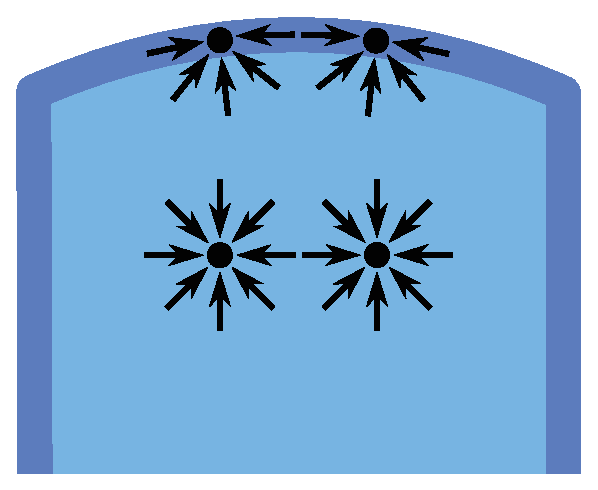
\includegraphics[width=10cm]{./figures/povrsinski_napon.eps}
              %\caption{Povr\v sinski napon}
              %\end{figure}
          \item[Gradijent] neke skalarne funkcije je vektorsko polje gde vektor u svakoj ta\v cki pokazuje u smeru najve\'ceg porasta, i ima intenzitet jednak tom porastu. Matemati\v cki, za funkciju $f(x, y, z)$:
                \begin{equation}\label{eq:definicija gradijenta}
                \nabla f=\frac{\partial f}{\partial x}\vec{i} + \frac{\partial f}{\partial y}\vec{j} + \frac{\partial f}{\partial z}\vec{k}
                \end{equation}
                pri \v cemu se $\vec{i}, \vec{j}, \vec{k}$ jedini\v cni vektori u tri dimenzije.
                %\begin{figure}[H]
                %\centering%
                %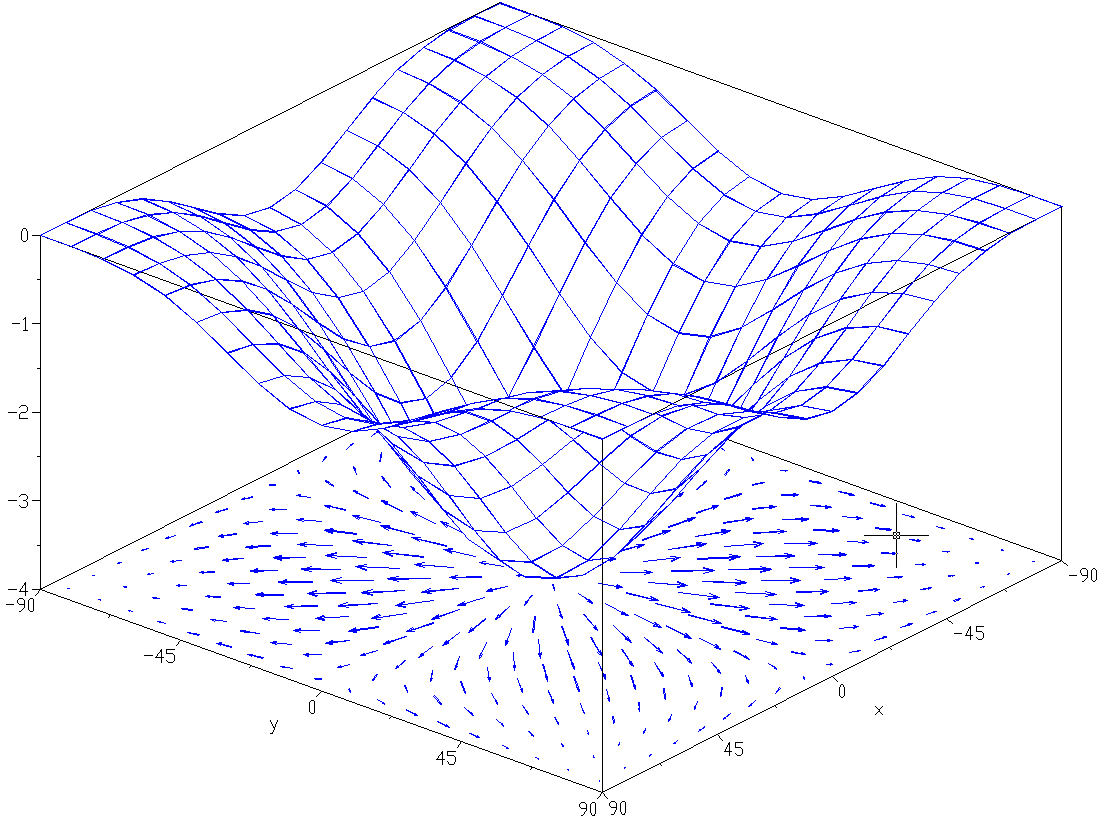
\includegraphics[width=10cm]{./figures/Gradient.png}
                %\caption{Povr\v sinski napon}
                %\end{figure}
          \item[Divergencija] vektorskog polja $\vec{v}(x, y, z)=v_x\vec{i}+v_y\vec{j}+v_z\vec{k}$ je skalarna funkcija
                \begin{equation}\label{eq:definicija divergencije}
                \text{div} \vec{v} = \nabla \cdot \vec{v} = \frac{\partial v_x}{\partial x} + \frac{\partial v_y}{\partial y} + \frac{\partial v_z}{\partial z}
                \end{equation}
          \item[Laplaceov operator] funkcije $f$ je divergencija gradijenta te funkcije.
          \begin{equation}\label{eq:definicija laplaceovog operatora}
          \nabla^2 f = \nabla\cdot\nabla f = \frac{\partial^2 f}{\partial x^2} + \frac{\partial^2 f}{\partial y^2} + \frac{\partial^2 f}{\partial z^2}
          \end{equation}
              Za neku ta\v cku $t$, ona predstavlja meru koliko se vrednost $f$ u ta\v ckama na sferi sa centrom u $t$ menja u odnosu na $f(t)$, ako polupre\v cnik sfere raste.
        \end{description}
    \subsection{Navier-Stokesova jedna\v cina} \label{Navier Stokes}
        U op\v stem slu\v caju, Navier-Stokesova jedna\v cina izgleda ovako:
        \begin{equation}\label{eq:Navier-Stokes opsti slucaj}
            \rho(\frac{\delta \vec{v}}{\delta t} + \vec{v} \cdot \nabla \vec{v}) = -\nabla p + \nabla \cdot \vec{T} + \vec{F}
        \end{equation}
        Ona u stvari predstavlja drugi Newtonov zakon za kretanje fluida. Tako\dj e, za potrebe ovog rada je dovoljna pojednostavljena verzija jedna\v cine, koja se odnosi na Newtonovske fluide, nesti\v sljivog toka. Njeno izvo\dj enje sledi.

        Krenimo od drugog Newtonovog zakona,
        \begin{equation}\label{eq:Newtonov 2. zakon}
            \vec{F}=m\vec{a}
        \end{equation}
        Zamenimo ubrzanje sa materijalnim izvodom brzine po vremenu ($\vec{a} = \frac{D\vec{v}}{Dt}$), a masu sa gustinom (posmatramo jedini\v cnu zapreminu):
        \begin{equation}\label{eq:Navier-Stokes izvodjenje 1}
            \vec{F}=\rho\frac{D\vec{v}}{Dt}=\rho(\frac{\delta \vec{v}}{\delta t} + \vec{v} \cdot \nabla \vec{v})
        \end{equation}
        Sa druge strane, sile koje deluju na fluid mo\v zemo da podelimo na unutra\v snje (viskozitet, povr\v sinski napon,...) i spolja\v snje (gravitacija,...). Za po\v cetak, neka je gravitaciona sila $\rho \vec{g}$ (opet, ovo nije sila u strogom smislu te re\v ci, ve\'c sila po jedinici zapremine)
        \begin{equation}\label{eq:Navier-Stokes izvodjenje 2}
            \rho \vec{g} + \vec{F}_{\text{unutra\v snje}}=\rho\frac{D\vec{v}}{Dt}=\rho(\frac{\delta \vec{v}}{\delta t} + \vec{v} \cdot \nabla \vec{v})
        \end{equation}
        \v Sto se ti\v ce unutra\v snjih sila, radi pojednostavljivanja jedna\v cina (pa samim tim i njihovog re\v savanja), u daljem tekstu \'ce se koristiti dve pretpostavke:
        \begin{enumerate}
          \item Fluid je Newtonovski
          \item Fluid ima nesti\v sljiv tok
        \end{enumerate}
        \v Cinjenica da je fluid Newtonovski nam govori da je viskoznost konstantna, odnosno ne zavisi od tangencijalnog napona u fluidu, a iz definicije nesti\v sljivog toka znamo da je divergencija polja brzina jednaka nuli ($\nabla \cdot \vec v = 0$). Zato, unutra\v snje sile mo\v zemo podeliti na one izazvane razlikom u pritiscima (normalni napon), i na viskozne sile izazvane razlikom u brzinama (tangencijalni napon)\cite{particle-fluids}. U ovom slu\v caju, sile izazvane razlikom pritisaka mo\v zemo modelirati negativnim gradijentom pritiska ($-\nabla p$), a viskozne sile sa $\eta\nabla\cdot\nabla\vec{v}=\eta\nabla^2\vec{v}$, i tako dobijamo kona\v cnu Navier-Stokesovu jedna\v cinu za Newtonovske fluide nesti\v sljivog toka:
        \begin{equation}\label{eq:Navier-Stokes za nn fluide}
         \underbrace{\rho}_{\text{gustina}} \overbrace{(\underbrace{\frac{\delta \vec{v}}{\delta t}}_{\text{ubrzanje deli\'ca fluida}} + \underbrace{\vec{v} \cdot \nabla \vec{v}}_{\text{konvektivno ubrzanje}})}^{\text{ubrzanje}} = \underbrace{-\nabla p}_{\text{gradijent pritiska}} + \underbrace{\eta\nabla^2\vec{v}}_{\text{viskozitet}} + \underbrace{\vec{F}}_{\text{spolja\v snje sile}}
        \end{equation}
\section{Smoothed particle hydrodynamics}
    Osnovu SPH-a \v cini kona\v can broj \v cestica jednakih masa, od kojih svaka predstavlja jedan deo ($V_i$) zapremine datog fluida.
    Glavna prepreka u svim Lagrangeovskim algoritmima za simuliranje fluida le\v zi u \v cinjenici da je za fizi\v cki potpuno vernu simulaciju potrebno simulirati prakti\v cno neograni\v cen broj \v cestica. SPH taj problem prevazilazi tako \v sto vrednost neke fizi\v cke veli\v cine $A$ u nekoj ta\v cki $\vec{r}$ interpolira iz diskretnog skupa ta\v caka (na pozicijama $\vec{r}_i$) za koje smo ve\'c izra\v cunali vrednost $A_i$.
    \begin{equation}\label{eq:SPH interpolacija}
        A_\text{interpolirano}(\vec{r}) = \sum_i{A_i V_i W(\vec{r}-\vec{r}_i, h)} = \sum_i{A_i \frac{m_i}{\rho_i} W(\vec{r}-\vec{r}_i, h)}
    \end{equation}
    Jasno je da svaka \v cestica u\v cestvuje u $A_\text{interpolirano}$ srazmerno svojoj zapremini $V_i=\frac{m_i}{\rho_i}$ i vrednosti funkcije $W$ na udaljenosti $\vec{r}-\vec{r}_i$ od date ta\v cke $\vec{r}$ ($h$ je konstanta o kojoj \'ce uskoro biti re\v ci).

    Funkcija $W(\vec{r}, h)$ je tzv. kernel za poravnavanje (smoothing kernel) sa $h$ kao radijusom poravnavanja i slu\v zi da "rasporedi" uticaj $A_i$ u okolini (odnosno na udaljenosti $|\vec{r}-\vec{r}_i|$) \v cestice u ta\v cki $\vec{r}_i$. Zna\v caj parametra $h$ je samo u tome \v sto funkcija $W$ za vrednosti $|\vec{r}-\vec{r}_i|$ ve\'ce od $h$ ima vrednost 0, odre\dj uju\'ci preciznost simulacije tako \v sto na \v cesticu u $\vec{r}$ deluju samo \v cestice koje su joj dovoljno blizu, tj. imaju dovoljno velik uticaj na nju. Tako\dj e, radi efikasnosti i jednostavnosti simulacije, kernel se obi\v cno bira da bude simetri\v can ($W(\vec{r}, h)=W(-\vec{r}, h)$) i normalizovan ($\int W(\vec{r})d\vec{r}=1$).

    Na primer, gustina neke \v cestice se pomo\'cu gorenavedene formule mo\v ze izraziti na slede\'ci na\v cin:
    \begin{equation}\label{eq:SPH interpolacija gustine}
    \rho_j=\sum_i{m_i \frac{\rho_i}{\rho_i} W(\vec{r}_j-\vec{r}_i, h)}=\sum_i{m_i W(\vec{r}_j-\vec{r}_i, h)}
    \end{equation}

    Da bismo mogli da izrazimo ostale \v clanove Naver Stokesove jedna\v cine, potrebni su nam oblici izraza za SPH interpolaciju za $\nabla A$ i $\nabla^2 A$. Na sre\'cu, oni se ne razlikuju mnogo od SPH izraza za interpolaciju same veli\v cine $A$:
    \begin{equation}\label{eq:SPH interpolacija gradijenta}
    \nabla A_\text{interpolirano}(\vec{r}) = \sum_i{A_i \frac{m_i}{\rho_i} \nabla W(\vec{r}-\vec{r}_i, h)}
    \end{equation}
    i analogno za $\nabla^2 A$:
    \begin{equation}\label{eq:SPH interpolacija Laplasovog operatora}
    \nabla^2 A_\text{interpolirano}(\vec{r}) = \sum_i{A_i \frac{m_i}{\rho_i} \nabla^2 W(\vec{r}-\vec{r}_i, h)}
    \end{equation}
    Sada imamo sve potrebne ''alate'' da izvedemo SPH jedna\v cine za ostale \v clanove Navier Stokesove jedna\v cine.
    \subsection{Pritisak}
        Koriste\'ci SPH interpolaciju, izraz za ''sile pritiska'' izgleda ovako:
        \begin{equation}\label{eq:SPH interpolacija sile pritiska (original)}
        \vec{F}_{\text{pritisak}_i} = -\nabla p(\vec{r}_i)=-\sum_j p_j \frac{m_j}{\rho_j}\nabla W(\vec{r}_i-\vec{r}_j, h)
        \end{equation}
        Na\v zalost, ovakav izraz za silu pritiska nije simetri\v can, tj. sila kojom \v cestica $i$ deluje na \v cesticu $j$ je razli\v cita od sile kojom \v cestica $j$ deluje na \v cesticu $i$ . Zato, u \cite{Desbrun96smoothedparticles:} je predlo\v zena jednostavna metoda kako da se prethodna jedna\v cina simetrizuje: gustina $\rho_j$ se zameni sa aritmeti\v ckom sredinom gustina $\rho_i$ i $\rho_j$:
        \begin{equation}\label{eq:SPH interpolacija sile pritiska (simetricno)}
        \vec{F}_{\text{pritisak}_i} = -\sum_j m_j \frac{p_i+p_j}{2\rho_j}\nabla W(\vec{r}_i-\vec{r}_j, h)
        \end{equation}
        Jedino ostaje kako izra\v cunati pritiske kod \v cestica $i$ i $j$, a odgovor na njega je dat u \cite{Muller:2003:PFS:846276.846298}, inspirisan osnovnom jedna\v cinom gasnog stanja za idealni gas pri konstantnoj temperaturi:
        \begin{equation}\label{eq:SPH racunanje pritiska}
        p = k(\rho-\rho_0)
        \end{equation}
        $\rho_0$ je konstanta nazvana ''gustina ostatka'' (rest density), i ne\'ce uticati na rezultuju\'ce sile (koje se zasnivaju na razlici pritisaka), ali \'ce zato (pozitivno) uticati na numeri\v cku stabilnost simulacije \cite{Muller:2003:PFS:846276.846298}.
    \subsection{Viskozne sile}
        Analogno izrazu za sile pritiska, dobijamo:
        \begin{equation}\label{eq:SPH interpolacija sile viskoziteta (original)}
        \vec{F}_{\text{viskozitet}_i} = \eta\nabla^2 \vec{v}(\vec{r}_i)=\eta\sum_j \vec{v}_j \frac{m_j}{\rho_j}\nabla^2 W(\vec{r}_i-\vec{r}_j, h)
        \end{equation}
        Ni ova jedna\v cina ne daje simetri\v cne sile izmedju \v cestica $i$ i $j$, pa je balansiramo zamenjivanjem $\vec{v}_j$ sa $\vec{v}_j-\vec{v}_i$, odnosno $\vec{v}_i-\vec{v}_j$:
        \begin{equation}\label{eq:SPH interpolacija sile viskoziteta (simetricno)}
        \vec{F}_{\text{viskozitet}_i}=\eta\sum_j m_j \frac{\vec{v}_j-\vec{v}_i}{\rho_j}\nabla^2 W(\vec{r}_i-\vec{r}_j, h)
        \end{equation}
        Ova smena je sa fizi\v cke ta\v cke gledi\v sta sasvim opravdana, jer viskozne sile zavise od relativnih brzina slojeva te\v cnosti, a ne njihove apsolutne vrednosti.
    \subsection{Povr\v sinski napon}
        Radi vernije simulacije te\v cnosti, potrebno je uvesti i silu povr\v sinskog napona, koja je odgovorna za razne pojave uklju\v cuju\'ci ''barice'' koje nastaju pri prosipanju te\v cnosti na neku podlogu, kapilarne efekte, ... Prirodno, da bismo izra\v cunali povr\v sinski napon, potrebno je prvo odrediti koje \v cestice su najbli\v ze povr\v sini. To se posti\v ze metodom ''polja boja'' (colour field), koja u ta\v ckama gde se nalaze \v cestice ima vrednost 1, a u ostalim 0. Naravno, ovakvo polje je nepogodno za rad, pa se zato koristi njegova poravnata varijanta, sli\v cna ostalim SPH formulama:
        \begin{equation}\label{eq:SPH interpolacija polja boja}
        c_S(\vec{r}) = \sum_i 1\cdot\frac{m_i}{\rho_i}W(\vec{r}-\vec{r}_i, h)
        \end{equation}
        Sada se vidi da \'ce ovakvo polje imati velik gradijent blizu povr\v sine (mnogo prelaza iz 1 u 0), i mali u unutra\v snjosti te\v cnosti (uglavnom vrednosti blizu 1). Po\v sto u povr\v sinskom naponu u\v cestvuje i zakrivljenost slobodne povr\v sine te\v cnosti, potrebno je izraziti i taj ugao zakrivljenosti:
        \begin{equation}\label{eq:SPH ugao zakrivljenosti}
        \kappa = \frac{-\nabla^2c_S}{|\nabla c_S|}
        \end{equation}
        Kombinuju\'ci ove jedna\v cine, dobijamo:
        \begin{equation}\label{eq:SPH interpolacija sile povrsinskog napona}
        \vec{F}_{\text{pov. napon}} = \sigma\kappa\nabla c_S = -\sigma \nabla c_S \frac{\nabla^2 c_S}{|\nabla c_S|}
        \end{equation}
    \subsection{Dodatne napomene}
        Kao \v sto je ve\'c nagove\v steno na po\v cetku dela \ref{Navier Stokes}, po\v sto se u SPH posmatraju nesti\v sljive \v cestice, mo\v zemo zanemariti advekciju, odnosno $\nabla \cdot \vec{v}=0$, Navier Stokesova jedna\v cina za ovakve \v cestice je:
        \begin{equation}\label{eq:Navier-Stokes pojednostavljeni}
        \rho \frac{\partial \vec{v}}{\partial t} = -\nabla p +\eta \nabla^2\vec{v}+\vec{F}
        \end{equation}
\section{Interakcija sa \v cvrstim telima}
    Interakcija sa \v cvrstim telima (u daljem tekstu: zidovima) je re\v sena na dva na\v cina: SPH i sudar \v cvrstih tela.
    \subsection{SPH na\v cin}\label{SPH sudari sa zidom}
        Iako ova metoda nije opisana nigde u literaturi, do nje se prirodno dolazi primenom SPH logike: zidovi se posmatraju kao da su i sami napravljeni od stati\v cnih \v cestica velike gustine. Naravno, ovakav na\v cin predstavljanja nije zgodan ni za ljudsku, ni za kompjutersku upotrebu. Zato, ljudi (korisnici) unose linije kao parove ta\v caka, a program implicitno pravi nove \v cestice u blizini podno\v zja normale iz \v cestice na zid. Zatim se te \v cestice zida normalno koriste u SPH jedna\v cinama za ra\v cunanje gustina, i sila koje deluju na \v cestice te\v cnosti. Prirodno, nisu nam bitne sile koje deluju na \v cestice zida, jer je pretpostavka da je zid stati\v can.
    \subsection{Sudar \v cvrstih tela} \label{Sudar cvrstih tela}
        Sa druge strane, ako i posle primene prethodnog algoritma postoji opasnost da \v cestica pro\dj e kroz zid, ovaj primitivni algoritam \'ce je odbiti kao gumenu lopticu, reflektovanjem vektora njene brzine u odnosu na zid. Ovo je poslednji deo svakog koraka simulacije, i izvr\v sava se sve dok tokom simuliranog vremena ($dt$) \v cestica ima u blizini zid kroz koji bi pro\v sla, a da nije prethodno bila odbijena od njega.

    \subsection{Pseudokod}

\begin{codebox}
\li \While \const{simulacija-radi} \Do
\li     \For $\id{i} \gets 1$ \To $\const{broj-\v cestica}$ \Do
\li          Postaviti $\id{\v cestica[i].gustina}$, $\id{\v cestica[i].pritisak}$, $\id{\v cestica[i].sila-pritiska}$, 
\zi          $\id{\v cestica[i].viskozna-sila}$, $\id{\v cestica[i].gradijent-polja-boja}$, 
\zi          $\id{\v cestica[i].Laplaceov-operator-polja-boja}$, $\id{\v cestica[i].sila-površinskog-napona}$, 
\zi          $\id{\v cestica[i].sila}$, $\id{\v cestica[i].ubrzanje}$ na 0
        \End
\li     \For $\id{i} \gets 1$ \To $\const{broj-\v cestica}$ \Do
\li         \For $\id{j} \gets 1$ \To $\const{broj-\v cestica}$ \Do
\li             \Comment Prema jedna\v cini~\eqref{eq:SPH interpolacija gustine}
\li             izra\v cunati gustine koje $\id{\v cestica}[i]$ i $\id{\v cestica}[j]$ dodaju jedna drugoj
            \End
\li         \For $\id{j} \gets 1$ \To $\const{broj-zidova}$ \Do
\li             \Comment Prema~\ref{SPH sudari sa zidom}
\li             izra\v cunati dodatnu gustinu za cesticu koju $\id{zid}[j]$ dodaje $\id{\v cestici}[i]$
            \End
        \End
\li     \For $\id{i} \gets 1$ \To $\const{broj-\v cestica}$ \Do
\li         \For $\id{j} \gets 1$ \To $\const{broj-\v cestica}$ \Do
\li             \Comment Prema jedna\v cinama ~\eqref{eq:SPH racunanje pritiska},~\eqref{eq:SPH interpolacija sile pritiska (simetricno)},~\eqref{eq:SPH interpolacija sile viskoziteta (simetricno)},~\eqref{eq:SPH interpolacija polja boja},~\eqref{eq:SPH interpolacija gradijenta},~\eqref{eq:SPH interpolacija Laplasovog operatora}
\li             izra\v cunati $\id{pritisak}$, dodatne $\id{sile-pritiska}$, $\id{viskozne-sile}$,
\zi             $\id{gradijent-polja-boja}$, $\id{Laplaceov-operator-polja-boja}$
\zi             koje $\id{\v cestica}[i]$ i $\id{\v cestica}[j]$ dodaju jedna drugoj
            \End
\li         \For $\id{j} \gets 1$ \To $\const{broj-zidova}$ \Do
\li             \Comment Prema~\ref{SPH sudari sa zidom}
\li             izracunati dodatne sile pritiska i viskoziteta
\zi             koje $\id{zid}[j]$ dodaje $\id{\v cestici}[i]$
            \End
        \End
\li     \For $\id{i} \gets 1$ \To $\const{broj-\v cestica}$ \Do
\li          \Comment Prema~\eqref{eq:SPH interpolacija sile povrsinskog napona}
\li          izra\v cunati $\id{silu-povr\v sinskog-napona}$ za $\id{\v cesticu}[i]$
\li          \Comment Prema~\eqref{eq:Newtonov 2. zakon}
\li          izra\v cunati $\id{ukupnu-silu}$, $\id{ubrzanje}$, $\id{novu-brzinu}$ i $\id{pomeraj}$
\li          \Comment Prema~\ref{Sudar cvrstih tela}
\li          odbiti $\id{\v cesticu}[i]$ od prepreka
        \End
\li     Iscrtati \v cestice na ekran
   \End
\end{codebox}
\emph{Napomena:} svaki put kada je neka vrednost izra\v cuna, ona se \v cuva kao odgovaraju\'ci atribut te \v cestice.

    \subsection{Tehi\v cki detalji}
        Naivna implementacija goreopisanog algoritma je naravno daleko od optimalne. Zato je kori\v s\'ceno nekoliko ''trikova'' za optimizaciju. Jasno je da u navedenom algoritmu najvi\v se vremena odlazi na operacije koje se odnose na svaki par \v cestica ($\mathcal{O}(n^2)$ vremena). Prime\'ceno je da od mogu\'cih $n^2$ parova \v cestica veliki broj njih uop\v ste ne uti\v ce jedna na drugu, jer su one na dovoljno velikoj udaljenosti da bi vrednost funkcije za poravnavanje bila $0$. Da bi se u\v stedelo na vremenu, \v cestice su podeljene u \'celije, te se onda samo proverava interakcija \v cestica u istim i susednim \' celijama. Potom, kada se na po\v cetku jednog koraka odrede \v cestice koje \'ce me\dj usobno interagovati se sa\v cuvaju u jednu listu koja se onda koristi do kraja tog koraka.

        Program je pisan u programskom jeziku C++. Za grafiku je kori\v s\'cena biblioteka SDL, koja se oslanja na OpenGL grafi\v cki sistem.
        Teren za simulaciju, kao i ostali parametri simulaciju su sa\v cuvani u JSON formatu, za \v cije je u\v citavanje kori\v s\'cena biblioteka Boost.

\section{Rezultati}
    Napravljeni program simulira do oko 10000 \v cestica proizvoljne te\v cnosti (ili gasa), zadate parametrima. Simulacija radi na 60fps, na Intelovom \v cetvorojezgarnom Core i7 procesoru. \v Cestice vizuelno zadovoljavaju\'ce reaguju me\dj usobno, kao i sa zidovima, sve dok simuluacija ne postane nestabilna. Tada \v cestice po\v cinju da se kre\'cu haoti\v cno, i zakon odr\v zanja energije prividno prestaje da va\v zi.
    \begin{figure}[H]
    \centering
    \begin{subfigure}[b]{0.49\textwidth}
        \centering
        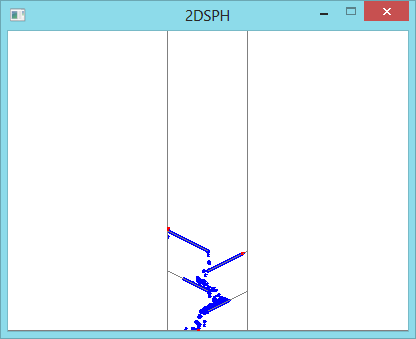
\includegraphics[width=\textwidth]{figures/screenshots/1.png}
        \caption{Stabilna simulacija}
        \label{fig:Stabilna simulacija}
    \end{subfigure}
    \begin{subfigure}[b]{0.49\textwidth}
        \centering
        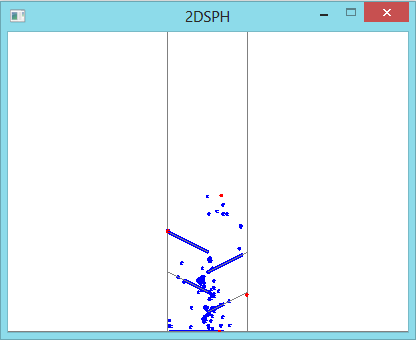
\includegraphics[width=\textwidth]{figures/screenshots/2.png}
        \caption{Nestabilna simulacija}
        \label{fig:Stabilna simulacija}
    \end{subfigure}
    \caption{Slike programa u radu} \label{Slike}
    \end{figure}
    Uzrok nestabilnosti jo\v s nije odre\dj en, ali verovatno le\v zi u lo\v sem izboru parametara simulacije. Eksperimenti pokazuju da je za to najzaslu\v zniji parametar ''gasna konstanta'', iz jedna\v cine \eqref{eq:SPH racunanje pritiska}. Ukoliko je on previ\v se mali, \v cestice se uop\v ste ne\'ce odbijati, a ukoliko je prevelik, simulacija postaje nestabilna. U ovom konkretnom slu\v caju, vrednost $k=250$ se pokazala skoro optimalnom.
\section{Zaklju\v cak}
    Iako simulacija daje vizualno prihvatljivi izlaz, zbog nepredvidivosti trenutka gubitka stabilnosti, jo\v s uvek nije pogodna za neku prakti\v cnu upotrebu.

    Dalji pravac razvoja bi verovatno i\v sao u smeru pove\'canja stabilnosti simulacije, kao i implementacija nekog naprednijeg algoritma za renderovanje fluida.

\newpage
\bibliographystyle{abbrv}
\bibliography{2DSPH}

\end{document}
